% DO NOT COMPILE THIS FILE DIRECTLY!
% This is included by the other .tex files.


\begin{frame}
    
\includegraphics[scale=.3]{images/logo-circl-Forensics.png}
    \begin{itemize}
        \item[]
        \item[]
        \item[] 13. Windows Registry
    \end{itemize}
\end{frame}


\begin{frame}[fragile]
  \frametitle{13.1 About: Windows Registry}
    \begin{itemize}
        \item MS DOS and old Windows
            \begin{itemize}
                \item On system boot: What programs to load
                \item How the system interact with the user
                \begin{itemize}
			\item[] $\to$ \texttt{autoexec.bat}
			\item[] $\to$ \texttt{config.sys}
			\item[] $\to$ \texttt{system.ini}
			\item[] $\to$ \texttt{win.ini}
                \end{itemize}
            \end{itemize}
        \item \url{https://support.microsoft.com/en-us/help/256986/}
            \begin{itemize}
                \item Replace text based config files
                \item A central hierarchical database
                \item Contains information for operating
                \begin{itemize}
                    \item Hardware in the system
                    \item All aspects of MS Windows
                    \item Installed applications
                    \item Each user
                \end{itemize}
            \end{itemize}
    \item[] $\to$ A gold mine for forensics
    \end{itemize}
\end{frame}


\begin{frame}[fragile]
  \frametitle{13.1 About: Windows Registry}
    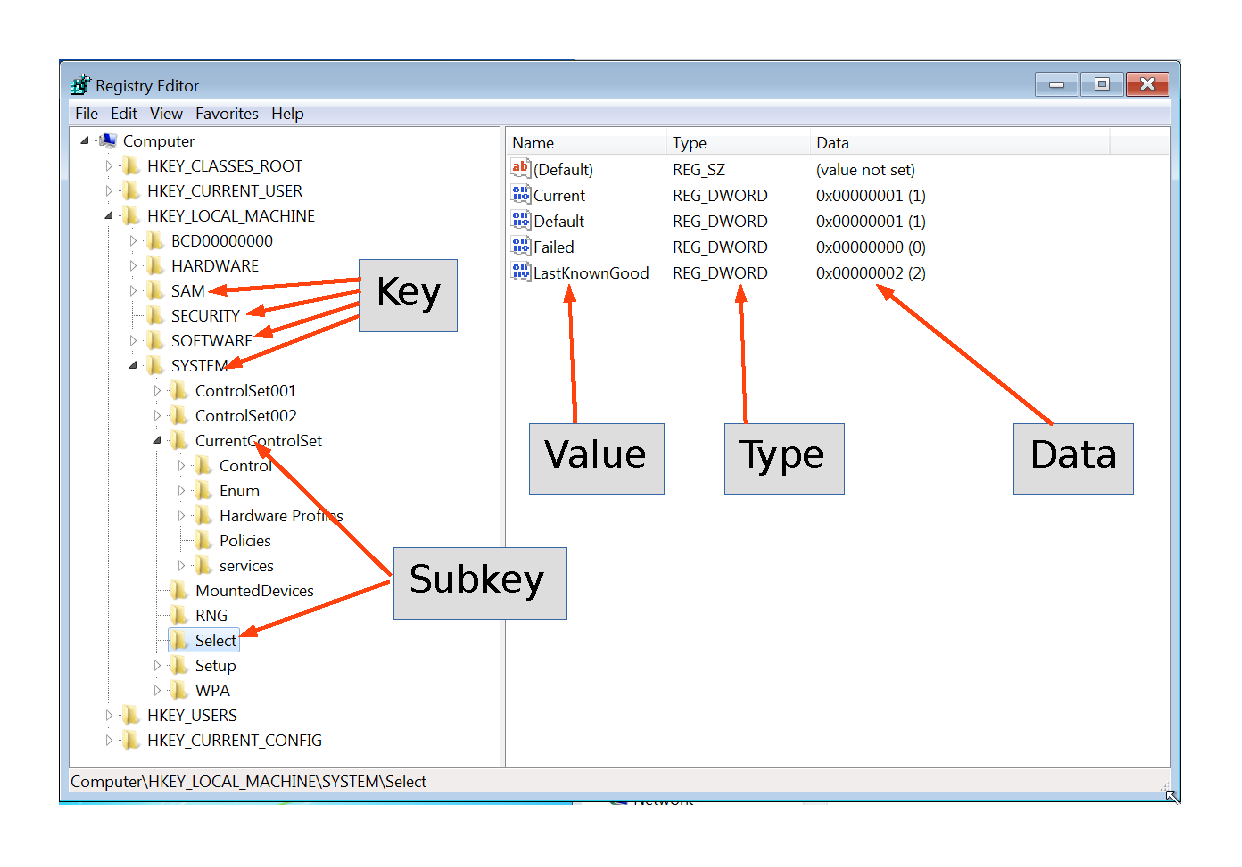
\includegraphics[scale=0.5]{images/nomenclature.pdf}
\end{frame}


\begin{frame}[fragile]
  \frametitle{13.1 About: Windows Registry}
    \begin{itemize}
        \item Do you ever touch the Registry?
            \begin{itemize}
		\item \texttt{regedit.exe}
                \item Black Magic for many admins
		\item[] $\to$ Every user interacts with the Registry
		\item[]
            \end{itemize}
        \item Location of the hive files
            \begin{itemize}
                \item[] \begin{verbatim}%SystemRoot%\system32\config\end{verbatim}
                \item[] $\to$ \texttt{SAM, SECURITY, SYSTEM, SOFTWARE}
                \item[] \begin{verbatim}%UserProfile%\NTUSER.DAT\end{verbatim}
                \item[] \begin{verbatim}%UserProfile%\AppData\Local\Microsoft\Windows\UsrClass.dat\end{verbatim}
		\item[]
            \end{itemize}
        \item Timestamps $\to$ Timeline
    \end{itemize}
\end{frame}


\begin{frame}[fragile]
  \frametitle{13.2 Under the hood: Key Cell}
  \definecolor{light-gray}{gray}{0.70}
  \begin{lstlisting}[basicstyle=\tiny,escapechar=§]
 §\colorbox{light-gray}{a0 ff ff ff}§ 6e 6b 20 00 6f 0f 0e 3b b7 8d d1 01  ....nk .o..;....
 02 00 00 00 08 5e 05 00 00 00 00 00 00 00 00 00  .....^..........
 ff ff ff ff ff ff ff ff 02 00 00 00 00 21 05 00  .............!..
 10 2e 00 00 ff ff ff ff 00 00 00 00 00 00 00 00  ................
 14 00 00 00 10 00 00 00 00 00 00 00 0a 00 00 00  ................
 49 6e 74 65 72 66 61 63 65 73 00 80 02 00 00 00  Interfaces......
  \end{lstlisting}
  \begin{lstlisting}[basicstyle=\tiny]
 Offsets in Bytes:       0       4        Size
                         4       2        Node ID
                         6       2        Node type
                         8       8        Last write time
                            ...
                        76       2        Lenght of key name
                        80     <76>       key name + padding
  \end{lstlisting}
  \begin{itemize}
      \item Exercise: Calculate the size of the key cell
      \begin{itemize}
          \item[] \texttt{a0 ff ff ff}
      \end{itemize}
      \item Exercise: Calculate the size of the key name
      \begin{itemize}
          \item[] \texttt{0a 00}
      \end{itemize}
  \end{itemize}
\end{frame}


\begin{frame}[fragile]
  \frametitle{13.2 Under the hood: Value Cell}
  \definecolor{light-gray}{gray}{0.70}
  \begin{lstlisting}[basicstyle=\tiny,escapechar=§]
                           §\colorbox{light-gray}{d8 ff ff ff}§ 76 6b 0d 00          ....vk..
 04 00 00 80 02 00 00 00 04 00 00 00 01 00 00 00  ................
 4c 61 73 74 4b 6e 6f 77 6e 47 6f 6f 64 00 00 00  LastKnownGood...
  \end{lstlisting}
  \begin{lstlisting}[basicstyle=\tiny]
 Offsets in Bytes:       0       4        Size
                         4       2        Node ID
                         6       2        Value name length
                         8       4        Data lenght
                        12       4        Data offset
                        16       4        value typw
  \end{lstlisting}
  \begin{itemize}
      \item Exercise: Calculate the size of the value cell
      \begin{itemize}
          \item[] \texttt{d8 ff ff ff}
      \end{itemize}
      \item Exercise: Calculate the size of the value name length
      \begin{itemize}
          \item[] \texttt{0d 00}
      \end{itemize}
  \end{itemize}
\end{frame}


\begin{frame}[fragile]
  \frametitle{13.3 Hive files}
   \begin{itemize}
       \item[]
   \begin{itemize}
      \item SAM hive
      \begin{itemize}
          \item Local users
      \end{itemize}
      \item Security hive
      \begin{itemize}
          \item Audit settings
          \item Machine, domain SID
      \end{itemize}
      \item System hive
      \begin{itemize}
          \item General system configuration
          \item Networking, Auto run
          \item Program execution
          \item USB devices
       \end{itemize}
      \item Software hive
      \begin{itemize}
          \item Windows version, Profiles list
          \item Networking, Auto run
          \item Shell extensions, Browser helper objects
          \item Scheduled Tasks
          \item Program execution
      \end{itemize}
   \end{itemize}
   \end{itemize}
\end{frame}


\begin{frame}[fragile]
  \frametitle{13.3 Hive files}
    \begin{itemize}
        \item Windows XP:
        \item[] \begin{verbatim}C:\Documents and Settings\<username>\NTUSER.DAT\end{verbatim}
        \item[] \begin{verbatim}C:\Documents and Settings\<username>\Local Settings\\end{verbatim}
        \item[] \begin{verbatim}   Application Data\Microsoft\Windows\UsrClass.dat\end{verbatim}
        \item[]
        \item Windows Vista and above:
        \item[] \begin{verbatim}C:\Users\<user>\NTUSER.DAT\end{verbatim}
        \item[] \begin{verbatim}C:\Users\<user>\AppData\Local\Microsoft\Windows\\end{verbatim}
        \item[] \begin{verbatim}   UsrClass.dat\end{verbatim}
        \item[]
        \item \begin{verbatim}C:\Windows\inf\setupapi.log\end{verbatim}
    \end{itemize}
\end{frame}


\begin{frame}[fragile]
  \frametitle{13.4 RegRipper}
  \begin{itemize}
      \item Extract specific key values
  \begin{lstlisting}[basicstyle=\tiny]
$ rip.pl -p compname -r SYSTEM
	ComputerName    = WIN7WS
	TCP/IP Hostname = Win7WS
  \end{lstlisting}
      \item Alternative method
  \begin{lstlisting}[basicstyle=\tiny]
$ wine rip.exe -p compname -r SYSTEM
	ComputerName    = WIN7WS
	TCP/IP Hostname = Win7WS
  \end{lstlisting}
      \item RegRipper plugins
  \begin{lstlisting}[basicstyle=\tiny]
$ ls -l /usr/share/regripper/plugins | wc -l
	362
  \end{lstlisting}
      \item Ripping hive files with profiles
  \begin{lstlisting}[basicstyle=\tiny]
$ rip.exe -f sam -r SAM > out/sam.txt
$ rip.exe -f security -r SECURITY > out/security.txt
$ rip.exe -f system -r SYSTEM > out/system.txt
$ rip.exe -f software -r SOFTWARE > out/software.txt
$ rip.exe -f ntuser -r NTUser.dat > out/ntuser.txt
$ rip.exe -f usrclass -r UsrClass.dat > out/userClass.txt
  \end{lstlisting}
  \end{itemize}
\end{frame}


\begin{frame}[fragile]
  \frametitle{13.5 RegRipper: Exercise}
  \begin{enumerate}
      \item Extract Hive files from invected PC
      \item Rip them with RegRipper profiles
      \item Collect important general information
      \item Try to find incident related artefacts
      \item Add the information to report
  \end{enumerate}
\end{frame}


\begin{frame}[fragile]
  \frametitle{13.6 Important user keys}
   \begin{itemize}
      \item AutoStart
      \begin{itemize}
          \item RunOnce
          \item Run
              \begin{itemize}
		      \item \texttt{\scriptsize{/Software/Microsoft/Windows/CurrentVersion/Run/}}
                  \item Executed at user login
                  \item Provide \(malware\) persistence
                  \item No admin privileges required
              \end{itemize}
          \item Much more... 
          \item Legacy and other AutoStart
              \begin{itemize}
		      \item \texttt{\scriptsize{/Software/Microsoft/Windows/CurrentVersion/Policies/Explorer/Run/}}
		      \item \texttt{\scriptsize{/Software/Microsoft/Windows NT/CurrentVersion/Windows/'load','run'}}
		      \item[]
              \end{itemize}
      \end{itemize}
      \item Program execution: By 'cmd.exe'
      \begin{itemize}
          \item MUI Cache
          \begin{itemize}
              \item XP: \texttt{\scriptsize{Software/Microsoft/Windows/ShellNoRoam/MUICache/}}
              \item Vista:  \texttt{\scriptsize{Local Settings/Software/Microsoft/Windows/Shell/MUICache/}}
          \end{itemize}
      \end{itemize}
   \end{itemize}
\end{frame}


\begin{frame}[fragile]
  \frametitle{13.6 Important user keys}
   \begin{itemize}
      \item Program execution
      \begin{itemize}
          \item UserAssist - Track user activities
              \begin{itemize}
		  \item \texttt{\scriptsize{/Software/Microsoft/Windows/CurrentVersion/Explorer/UserAssist/}}
		  \item \texttt{\scriptsize{rip.pl -r john.dat -p userassist | less}}
		  \item 'Windows Explorer Shell' \& 'START menu' users interaction
                  \item Subkey values: Path, Run-Count, FileTime last access
                  \item Subkey values: ROT-13
              \end{itemize}
          \item Application Compatibility Assistant
	  \item[]
      \end{itemize}
      \item File-, Folder-, Share access
      \begin{itemize}
          \item Shell Bags
              \begin{itemize}
                  \item Track views, sizes and positions of a folders
                  \item Incl. time stamps
		  \item Incl. ZIP subfolders \& IE FTP
              \end{itemize}
          \item MRU Lists
              \begin{itemize}
		  \item \texttt{RecentDocs}
		  \item \texttt{RunMRU}
              \end{itemize}
      \end{itemize}
   \end{itemize}
\end{frame}


\begin{frame}[fragile]
  \frametitle{13.6 Important user keys}
   \begin{itemize}
      \item File access
      \begin{itemize}
          \item RecentDocs
          \begin{itemize}
              \item[] Example: '.png' files
                  \begin{lstlisting}[basicstyle=\tiny]
Software\Microsoft\Windows\CurrentVersion\Explorer\RecentDocs\.png
LastWrite Time Fri Jan 12 15:00:52 2018 (UTC)
MRUListEx = 3,2,0,1
  3 = photo-123.png
  2 = paint.png
  0 = face.png
  1 = flower.png
                  \end{lstlisting}
          \end{itemize}

          \item Common Dialogs
          \begin{itemize}
              \item[] Example: 'Open' and 'Save As...'
                  \begin{lstlisting}[basicstyle=\tiny]
OpenSavePidlMRU\exe
LastWrite Time: Tue Jul  5 14:40:46 2016
Note: All value names are listed in MRUListEx order.

  Users\avast_free_antivirus_setup_online.exe
  Users\Thunderbird Setup 45.1.1.exe
  Users\Firefox Setup Stub 47.0.1.exe
                  \end{lstlisting}
          \end{itemize}
      \end{itemize}
   \end{itemize}
\end{frame}








